%%%%%%%%%%%%%%%%%%%%%%%%%%%%%%%%%%%%%%%%
%% MCM/ICM LaTeX Template %%
%% 2024 MCM/ICM           %%
%%%%%%%%%%%%%%%%%%%%%%%%%%%%%%%%%%%%%%%%
\documentclass[12pt]{article}
\usepackage{geometry}
\geometry{left=1in,right=0.75in,top=1in,bottom=1in}

%%%%%%%%%%%%%%%%%%%%%%%%%%%%%%%%%%%%%%%%
% Replace ABCDEF in the next line with your chosen problem
% and replace 1111111 with your Team Control Number
\newcommand{\Problem}{ABCDEF}
\newcommand{\Team}{1111111}
%%%%%%%%%%%%%%%%%%%%%%%%%%%%%%%%%%%%%%%%

\usepackage{newtxtext}
\usepackage{amsmath,amssymb,amsthm}
\usepackage{newtxmath} % must come after amsXXX

\usepackage[pdftex]{graphicx}
\usepackage{xcolor}
\usepackage{fancyhdr}
\usepackage{booktabs}
\usepackage{subcaption}
\lhead{Team \Team}
\rhead{}
\cfoot{}

\newtheorem{theorem}{Theorem}
\newtheorem{corollary}[theorem]{Corollary}
\newtheorem{lemma}[theorem]{Lemma}
\newtheorem{definition}{Definition}

%%%%%%%%%%%%%%%%%%%%%%%%%%%%%%%%
\begin{document}
\graphicspath{{.}}  % Place your graphic files in the same directory as your main document
\DeclareGraphicsExtensions{.pdf, .jpg, .tif, .png}
\thispagestyle{empty}
\vspace*{-16ex}
\centerline{\begin{tabular}{*3{c}}
	\parbox[t]{0.3\linewidth}{\begin{center}\textbf{Problem Chosen}\\ \Large \textcolor{red}{\Problem}\end{center}}
	& \parbox[t]{0.3\linewidth}{\begin{center}\textbf{2024\\ MCM/ICM\\ Summary Sheet}\end{center}}
	& \parbox[t]{0.3\linewidth}{\begin{center}\textbf{Team Control Number}\\ \Large \textcolor{red}{\Team}\end{center}}	\\
	\hline
\end{tabular}}
%%%%%%%%%%% Begin Summary %%%%%%%%%%%
% Enter your summary here replacing the (red) text
% Replace the text from here ...
\begin{center}
\textcolor{red}{%
Use this template to begin typing the first page (summary page) of your electronic report. This \newline
template uses a 12-point Times New Roman font. Submit your paper as an Adobe PDF \newline
electronic file (e.g. 1111111.pdf), typed in English, with a readable font of at least 12-point type.	\\[2ex]
Do not include the name of your school, advisor, or team members on this or any page.	\\[2ex]
Papers must be within the 25 page limit.	\\[2ex]
Be sure to change the control number and problem choice above.	\\
You may delete these instructions as you begin to type your report here. 	\\[2ex]
\textbf{Follow us @COMAPMath on Twitter or COMAPCHINAOFFICIAL on Weibo for the \newline
most up to date contest information.}
}
\end{center}
% to here
%%%%%%%%%%% End Summary %%%%%%%%%%%

%%%%%%%%%%%%%%%%%%%%%%%%%%%%%%
\clearpage
\pagestyle{fancy}
% Uncomment the next line to generate a Table of Contents
%\tableofcontents 
\newpage
\setcounter{page}{1}
\rhead{Page \thepage\ }
%%%%%%%%%%%%%%%%%%%%%%%%%%%%%%

\begin{equation}
		PPPM = \textbf{W}^{\top}\cdot\textbf{I}=
		\begin{pmatrix}
			\sigma_1 & \sigma_2 & \sigma_3 & \sigma_4
		\end{pmatrix}\cdot\begin{pmatrix}
		MW & IWW & AAP & GT
		\end{pmatrix}^{\top}. 
	\label{map}
\end{equation}

\begin{equation}
	\textbf{I} =  \textbf{T}(\cdot)=\begin{pmatrix}
	\alpha(t) \\ \beta(t) \\ \theta(t) \\ \gamma(t)
\end{pmatrix}=
\begin{pmatrix}
	-0.0481\times t+97.3493 \\ 0.0503\times t -100.6650 \\ 0.0355\times t-70.7723 \\ 0.0386\times t-76.9758
\end{pmatrix}
\end{equation}

since we applied the MLP as the backbone model, weight matrix have to be calculated as :

% MLP的原理
\begin{equation}
	\begin{cases}
		\textbf{O} =\mu(\textbf{W}_1\cdot\textbf{X}+\textbf{b})  \\
		\hat{\textbf{Y}} = \textbf{W}_2\cdot\textbf{O} +\textbf{b}
	\end{cases},\hspace{0.3em}\text{where}\hspace{0.3em}\mu(\cdot)\hspace{0.3em}=\mathrm{ReLU(\cdot)}
\end{equation}

% 计算权重的方法
\begin{equation}
	\hat{\textbf{Y}}=\textbf{W}_2\cdot\mu\cdot(\textbf{W}_1\cdot\textbf{X}+\textbf{b})=\textbf{W}_{\text{total}}\cdot\textbf{X}+\textbf{b}_{\text{total}}
\end{equation}
where:
\begin{equation}
	\textbf{W}_{\text{total}}=\textbf{W}_2\cdot\mu(\cdot)\cdot\textbf{W}_1=\begin{pmatrix}
		\varepsilon_{1} & \varepsilon_{2}
	\end{pmatrix}\cdot\begin{pmatrix}
	\mu(x_i)' & 0 & 0 & 0 \\
	0 &\mu(x_i)'  &0 & 0 \\
	0  & 0 &\mu(x_i)' &0 \\
	0 & 0 & 0 & \mu(x_i)'
	\end{pmatrix}\cdot\begin{pmatrix}
		\omega_{11} & \dots & \omega_{14}| \\
	\omega_{21} &  \dots & \omega_{24}
	\end{pmatrix}
\end{equation}
through training we have:
\begin{equation}	\textbf{W}_2=
\begin{pmatrix}
	-0.48617& 0.47315
\end{pmatrix},\hspace{0.2em}\textbf{W}_1 =\begin{pmatrix}
	0.31434 & -0.27920 & -0.15085 & -0.18880 \\
	-0.31076 & 0.26576 & 0.14595 & 0.18557 
\end{pmatrix}
\end{equation}
Hence, 
\begin{equation}
\textbf{W}^{\top} = \begin{pmatrix}
	-0.29985 & 0.26148 & 0.14239 & 0.17959
\end{pmatrix}\approx\begin{pmatrix}
-0.30 & 0.26 & 0.14 & 0.18
\end{pmatrix}
\end{equation}
then we have:
\begin{equation}
	PPPM = -0.3\times MW + 0.26\times IWW + 0.14\times AAP + 0.18\times GT
\end{equation}
if being mapped into the time dimension, then we have:
\begin{equation}
	PPPM = 0.039\times t -79.14
\end{equation}
where t stands for years and PPPM is a dimensionless variable which reflects the annual profits of construction projects. If PPPM > 0, then any construction projects can make profits without destroying the environments. Contrarily, if PPPM<0, it may destroy the environments while carrying out the project.

To give this equation stronger practical significance, we introduced "time coefficient" which describes the starting date of a project, which goes as :
\begin{equation}
	PPPM = 0.039\times(t+t_0)-79.14
\end{equation}

From this end, $t$ stands for the lasting time of a specified project. Therefore, the optimized model goes as:
\begin{equation}
	PPPM=0.039\times(t_0+\Delta t)-79.54
\end{equation} 
Similarly, if PPPM > 0, it can make profits without destroying the environment.
\begin{figure}[h]
	\centering
	\begin{subfigure}{0.2\textwidth}
		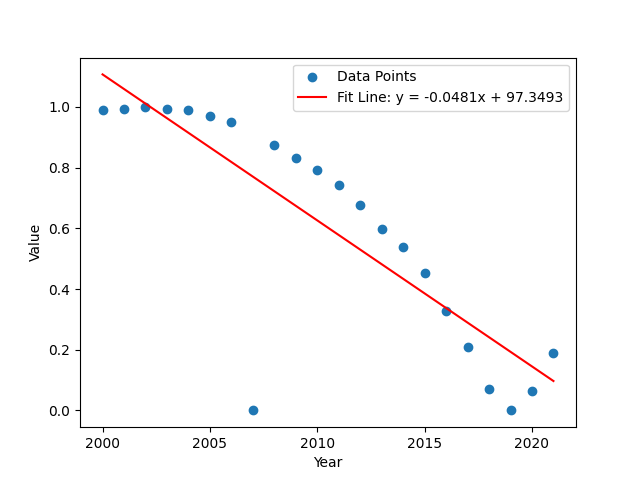
\includegraphics[width=\textwidth]{./figures/alpha_(t).png}
		\caption{$\alpha(t)$}
	\end{subfigure}
	\begin{subfigure}{0.2\textwidth}
	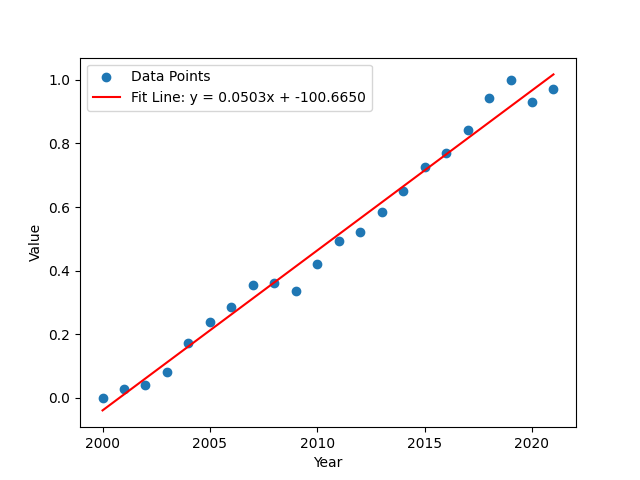
\includegraphics[width=\textwidth]{./figures/beta_(t).png}
	\caption{$\beta(t)$}
\end{subfigure}
	\begin{subfigure}{0.2\textwidth}
	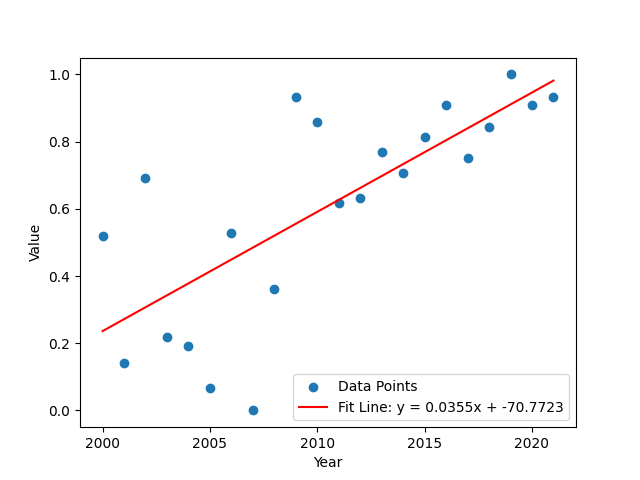
\includegraphics[width=\textwidth]{./figures/theta_(t).png}
	\caption{$\theta(t)$}
\end{subfigure}
	\begin{subfigure}{0.2\textwidth}
	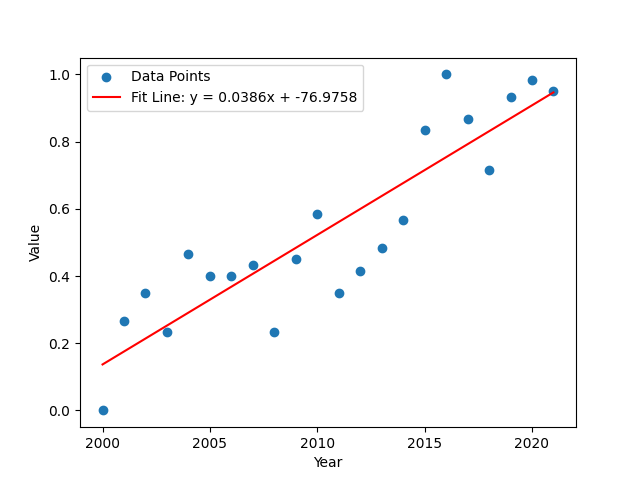
\includegraphics[width=\textwidth]{./figures/gamma_(t).png}
	\caption{$\gamma(t)$}
\end{subfigure}
\caption{Visualization of the linear fitting process.}
\end{figure}

%%%%%%%%%%%%%%%%%%%%%%%%%%%%%%
\end{document}
\end
